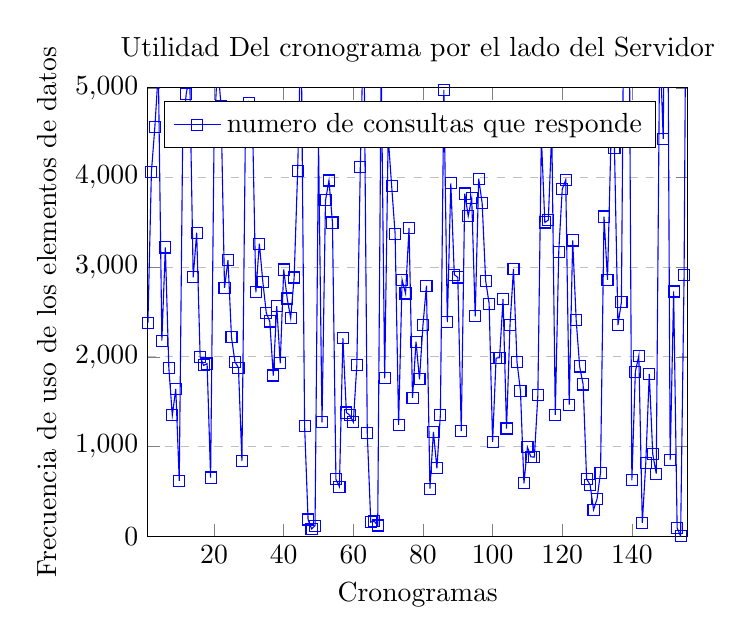
\begin{tikzpicture}
\begin{axis}[
    title={Utilidad Del cronograma por el lado del Servidor},
    xlabel={Cronogramas},
    ylabel={Frecuencia de uso de los elementos de datos},
    xmin=1, xmax=156,
    ymin=0, ymax=5000,
    xtick={},
    ytick={},
    legend pos=north west,
    ymajorgrids=true,
    grid style=dashed,
]

\addplot[
    color=blue,
    mark=square,
    ]
    coordinates {
%UTILIDAD TOTAL
%(cronograma, numero cues que usan al cronograma)
(1,2379)
(2,4062)
(3,4568)
(4,5195)
(5,2181)
(6,3220)
(7,1879)
(8,1348)
(9,1642)
(10,618)
(11,4523)
(12,4933)
(13,5152)
(14,2887)
(15,3384)
(16,1999)
(17,1905)
(18,1925)
(19,654)
(20,4465)
(21,5283)
(22,4799)
(23,2769)
(24,3079)
(25,2219)
(26,1943)
(27,1880)
(28,838)
(29,4550)
(30,4831)
(31,4704)
(32,2719)
(33,3263)
(34,2838)
(35,2488)
(36,2395)
(37,1792)
(38,2566)
(39,1929)
(40,2974)
(41,2651)
(42,2434)
(43,2885)
(44,4069)
(45,5713)
(46,1232)
(47,186)
(48,81)
(49,118)
(50,4397)
(51,1269)
(52,3745)
(53,3967)
(54,3498)
(55,634)
(56,553)
(57,2210)
(58,1379)
(59,1348)
(60,1272)
(61,1907)
(62,4114)
(63,5824)
(64,1153)
(65,157)
(66,167)
(67,119)
(68,5293)
(69,1761)
(70,4460)
(71,3909)
(72,3371)
(73,1242)
(74,2861)
(75,2707)
(76,3439)
(77,1542)
(78,2170)
(79,1749)
(80,2355)
(81,2794)
(82,530)
(83,1164)
(84,756)
(85,1355)
(86,4977)
(87,2388)
(88,3935)
(89,2917)
(90,2886)
(91,1172)
(92,3821)
(93,3570)
(94,3769)
(95,2452)
(96,3987)
(97,3714)
(98,2850)
(99,2594)
(100,1051)
(101,1986)
(102,1991)
(103,2646)
(104,1201)
(105,2356)
(106,2982)
(107,1943)
(108,1621)
(109,589)
(110,993)
(111,885)
(112,882)
(113,1573)
(114,4459)
(115,3499)
(116,3525)
(117,4533)
(118,1352)
(119,3173)
(120,3869)
(121,3974)
(122,1467)
(123,3298)
(124,2412)
(125,1893)
(126,1692)
(127,640)
(128,573)
(129,295)
(130,416)
(131,709)
(132,3565)
(133,2858)
(134,4429)
(135,4334)
(136,2355)
(137,2612)
(138,7654)
(139,7599)
(140,622)
(141,1834)
(142,2013)
(143,148)
(144,818)
(145,1810)
(146,914)
(147,698)
(148,5563)
(149,4430)
(150,8512)
(151,848)
(152,2729)
(153,93)
(154,0)
(155,2909)
(156,9185)
(157,7124)
    };
    \legend{numero de consultas que responde}

\end{axis}
\end{tikzpicture}

